\documentclass[11pt]{book}
% === core_packages.tex ===
\usepackage{amsmath, amssymb, amsthm, amsfonts}
\usepackage{geometry}
\usepackage{hyperref}
\usepackage{bookmark}
\usepackage{graphicx}
\usepackage{physics}
\usepackage{booktabs}
\usepackage{listings}
\usepackage{amscd}
\usepackage{tikz-cd}
\usepackage{mathtools}
\usepackage{xspace}
\usepackage[backend=biber, style=numeric]{biblatex}
\usepackage{tcolorbox}
\tcbuselibrary{theorems}
\usepackage{parskip}
\usepackage{tikz}
\usepackage{etoolbox}
\usetikzlibrary{arrows.meta, shapes, positioning, calc, cd, shapes.geometric, backgrounds}
\usepackage[en-US]{datetime2}
\usepackage{array}

% --- Theory names ---
\newcommand{\iame}{[theory needs name]}
\newcommand{\iameverything}{[theory needs name]}
\newcommand{\theory}{[theory needs name]}


% --- Math & Ontology Macros ---
\newcommand{\entropy}{S}
\newcommand{\opponent}{opponent}
\newcommand{\aside}[1]{[\emph{\opponent}: ``#1'']}
\newcommand{\paper}[1]{[\emph{#1}: ``#1'']}
\newcommand{\fabric}{voxel}
\newcommand{\Fabric}{Voxel}
\newcommand{\pdflink}[1]{}



% --- Global Layout Defaults ---
\geometry{letterpaper, margin=1in}
\hypersetup{
    colorlinks=true,
    linkcolor=black,
    citecolor=black,
    filecolor=magenta,
    urlcolor=blue
}
\hfuzz=5pt \vfuzz=5pt \hbadness=10000 \vbadness=10000

\author{\iame}

% === book_preamble.tex ===

% --- Book Specific Theorems (Numbered by Chapter) ---
\newtheorem{lemma}{Lemma}[chapter]
\theoremstyle{definition}
\newtheorem{axiom}{Axiom}[chapter]
\newtheorem{theorem}{Theorem}[chapter]
\newtheorem{corollary}{Corollary}[chapter]
\newtheorem{definition}{Definition}[chapter]
\newtheorem{proposition}{Proposition}[chapter]
\newtheorem{conjecture}{Conjecture}[chapter]

\makeatletter
\let\remark\@undefined
\let\endremark\@undefined
\makeatother
\theoremstyle{remark}
\newtheorem*{remark}{Remark}

% Theorem numbering tracks chapters cleanly here
\newtcbtheorem[number within=chapter]{principle}{Principle}%
{colback=blue!5,colframe=blue!50!black,fonttitle=\bfseries}{principle}

% --- Profilation ---
\newtoggle{theology}
\toggletrue{theology}   % default
\providecommand{\buildtheology}{true}
\ifdefstring{\buildtheology}{true}
  {\toggletrue{theology}}
  {\togglefalse{theology}}



\graphicspath{{cover/}{chapters/}{chapters/figures/}}

\begin{document}

\begin{titlepage}
\begin{tikzpicture}[remember picture,overlay]
\node[anchor=south] at (current page.south) {%
  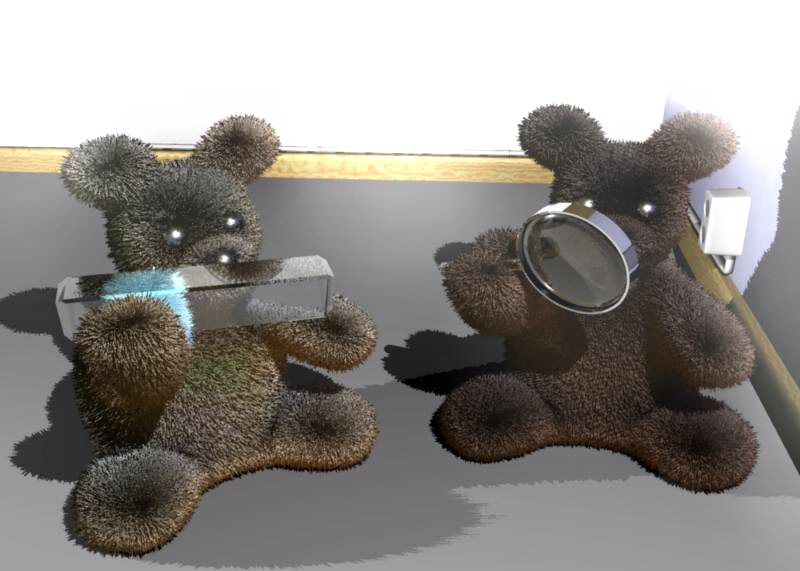
\includegraphics[
    width=\paperwidth,
    height=0.80\paperheight,
  ]{cover.jpg}
};
\end{tikzpicture}

\centering
{\Huge\bfseries Introduction to 184\par}

\vspace{1cm}
{\Large Juha Meskanen\par}
\vspace{0.5cm}

{\small\scshape Physics Edition\par}

\vspace{0.2cm}

{\footnotesize\ttfamily [ Code: 184 ]\par}


\end{titlepage}

\newpage
\thispagestyle{empty} % No headers or footers
\vspace*{\fill}       % Push content to the bottom

\begin{flushleft}
    \small
    
    \textit{Build: \DTMnow}

    
    \vspace{1.5em} % Some breathing room
    
    Draft Edition \\
    \textbf{Copyright \textcopyright\ 2001--2026 Juha Meskanen} \\
    All rights reserved.
\end{flushleft}
\newpage




\tableofcontents

\mainmatter
\chapter{History of the Abstract Universe Project}
\label{chap:history}

\section*{Introduction}

This chapter follows a journal-style structure, tracing the project in chronological order year by year.
It seeks to illuminate how the framework originated and evolved, from its initial spark to its current state.

Working on this project has brought both immense satisfaction and deep frustration, operating in predictable cycles,
where the latter inevitably follows the former.
Perhaps the central discovery of the entire journey is simply an appreciation for the sheer, staggering complexity of everything.


\section*{History}

\begin{description}

\item[\textbf{1988}: Pain]
  The "tooth ache" cache incident ignites long discussions with colleagues on whether pain could ever be implemented as software.

\item[\textbf{1989}: Abstract Nature of Everything]
  First simulated human thought experiment: discovering that simulated humans would also discover they can duplicate their structure in a Turing machine. We did!

  Conclusion: the simulation software is recursive. There is no single additional variable between two recursion levels that would make the simulated virtual human any less real (or us any more real). Since we know the simulated human is virtual, so must we be.

  Vesa's discovery: by observing such a simulation, we would notice that simulated humans start extracting information from their spatial surroundings; they are building a Turing machine to simulate themselves!

  The universe must be abstract by nature.

\item[\textbf{1989}: The Source of Pain Mystery]
  If millions of lines of code create a suffering virtual human, what is the exact source of that suffering? Is it when the CPU moves data from memory to an internal register, or when it flips a bit?

  Realization: any computer can be implemented as a mechanical device using wooden spheres passing through wooden gates. If a vast network of wooden components creates a suffering virtual human, what does a single moving wooden component create?

  Is this \textbf{real} $\rightarrow$ \textbf{virtual} action beyond known physics?

\item[\textbf{1991}: Major Breakthrough: Human as an Axiomatic System]
  The discovery that DNA can be digitized and simulated in a digital system. Two observational assumptions serve as axioms: DNA contains the instructions on how to build pain, and no magic plays a role in its operation, it consists of ordinary particles operating according to the laws of physics.

  The laws of physics are based on mathematics, and mathematics is an axiomatic system. A human must therefore be entirely an axiomatic system. A Turing machine is an implementation of an axiomatic system; therefore, a human can be simulated.

\item[\textbf{1992}: Pain Hypothesis]
  Discovery that pain has measurable effects. A human in pain is physically distinct from a human without pain. The influence of pain can be measured just like the effects of gravity.

  Conclusion: simulated humans must feel pain, or there would be a mathematical contradiction, two identical axiomatic systems would behave differently. $2+2$ with bananas would not equal $2+2$ with apples.


\item[\textbf{1994} -- Theory of Morality and God]

  Viewing the human as an axiomatic system raises an unsettling question regarding free will and God.

  Thesis of Morality: what we define as ``right'' aligns precisely with the typical evolutionary behaviors of group-living social animals.  

  Thesis of God: we believe in God because we are social animals whose survival depends on group organization. Humans utilize the concept of leadership to maintain order, and God represents the ultimate, idealized leader. Evolution has burned
  us tendency to follow good leaders, and God represents the ultimate, idealized leader.
  
  
\item[\textbf{1993}: The Method]
  We do not know the true nature of time or a black hole singularity. However, we can simulate them. Whatever they are, their functional equivalents must exist inside the computer running the simulation. Therefore, we can study the computer, whose internal structure we perfectly understand.

\item[\textbf{1994}: The Two Time Thought Experiments]
  Discovery: time can be gradually optimized out by replacing simulation code with static data. A simulated human must still experience pain, otherwise there would be a code/data threshold where pain vanishes. Consciousness must emerge from static data.

  Derived thought experiment: in a multithreaded, preemptive computer system, consciousness inevitably emerges from pure white noise.

  The fundamental nature of the universe is static, timeless, random \textbf{noise}.

  \textit{How could gravity possibly work in static random noise?}

\item[\textbf{1995}: Collapsing Spacetime and the Equivalence of Singularity and Entropy]
  First gravity thought experiment monitoring a black hole simulation of collapsing spacetime and the entropy of its memory image. Discovery: entropy decreases as spacetime collapses. Although the simulation crashes before the singularity forms, we can extrapolate the entropy trend: a singularity is a zero-entropy state.

  Discovery: any attempt to interpret zero-entropy information as geometric space always maps to a single object, a geometric point.

\item[\textbf{1996}: Time-Reversed Black Hole Thought Experiment]
  Discovery that all geometric interpretations of increasing entropy yield an expanding universe.

  Hypothesis: an expanding universe and increasing entropy are two sides of the same coin.

  Inflationary expansion of the early universe: a random system rushing from zero entropy toward thermodynamic equilibrium.

\item[\textbf{1996}: Major Frustration: Emergence of Gravity]
  First actual simulations written in C/C++ demonstrate exploding, expanding dust clouds.

  The probability of emergent structure is practically zero.

  \textit{How could gravity possibly emerge within this framework?}

\item[\textbf{2001}: Increasing Entropy and Emergent Geometric Microstructures]
  Simulations mapping increasing entropy to geometric space while filtering microstructures reveal a log-normal distribution curve. The probability of emergent structure appears to follow a log-normal shape.

\item[\textbf{2005}: Box of Coins Experiment]
  Major discovery via the "coins in a box" thought experiment: the more ways coins can be arranged to describe a structure, the higher the probability of that structure emerging.

  How do we maximize the probability of emergence? By using some of the bits to describe a compression algorithm!

  A random emergent observer will most likely find themselves residing within a compressed structure.

\item[\textbf{2006}: Gravity, Finally]
  Predictable, smoothly evolving data compresses far better than chaotically jumping data: enter mass and inertia!

  We most likely find ourselves in a smoothly evolving, predictable universe because predictable information compresses best. That is precisely what the laws of physics represent: predictability.

\item[\textbf{2009}: Complex-Valued Wavefunction as Compression]
  Discovery that waves permeate the microcosm everywhere, we are observing compressed structure. The quantum mechanical complex-valued wavefunction is the universe's compression signature; the Born rule acts as its dithering system.

  Thought experiment: render all possible videos of yourself in all possible formats, both compressed and uncompressed. Pick one at random. What do you observe? Most likely a dithered, compressed video, because bits can be arranged to render you in vastly more ways through compression and dithering.

\item[\textbf{2010}: Black Hole Simulation]
  First serious simulation proof-of-concept demonstrating the vanishing entropy and geometric singularity hypothesis, accompanied by a semi-formal paper draft.

  Conclusions: a spacetime singularity is a zero-information state. No information, no probability of emergent particles, no spacetime curvature.

\item[\textbf{2011}: First Simulation of Emergent Gravity]
  First attempts to develop minimal toy simulations showing how physical laws can emerge simply by randomly selecting execution frames representing an evolving minimal structure (e.g., a Gaussian blob).

  Conclusion: the most compressible state histories of a Gaussian blob are the most numerous, demonstrating emergent inertia.

\item[\textbf{2012}: Emergence of Spacetime]
  First simulations demonstrating the time-reverse of a black hole: the emergence of spacetime, accompanied by a paper draft.

\item[\textbf{2014}: The Book: \textit{Good Heavens Gods? Hell No Dogs!}]
  First draft of the manuscript takes shape after an intense two-year effort.

  What's a good title for a book like this? \textit{Good Heavens Gods? Hell No Dogs!}

\item[\textbf{2018}: Why Geometry? Why Not High-Dimensional Spectral?]
  Realization: we perceive life in a geometric $3+1$ spacetime. Why geometric? Why not a high-dimensional complex-valued spectral representation in Hilbert space?

  We require well-defined inside/outside boundaries to prevent our information from leaking and mixing with the environment. Any random, extraneous information injected outside degrades compression, leading to an exponentially vanishing probability of emergence.

  Idea: General Relativity (GR) might also be about compression, a minimal description required to define informational boundaries.

  Perhaps GR and Quantum Mechanics (QM) can be unified through compression!

\item[\textbf{2019}: The Consciousness Breakthrough]
  Discovery: different optimizations of a DNA simulation result in drastically different execution traces. A simulated human is not a single specific bit sequence, but an entire equivalence class of them. This is the fundamental definition of entropy.

  If simulated consciousness emerges from a sequence of bits, we face a dilemma: either the initial axioms about DNA are wrong, or everything we observe, including pain, must emerge from bit sequences.

  Breakthrough: in a static, timeless universe, there is no external "interpreter," and raw bits do not dictate how they should be decoded (e.g., two's complement). Only a vanishingly small fraction of possible interpretations map to a Turing machine.

  Pain has no room to operate within the strict confines of a Turing machine subset. However, pain has immense room to operate \textit{outside} that subset.

  Pain may be a heuristic navigation system operating on a vast "interpretation space," where strict algorithmic methods would be far too inefficient.

\item[\textbf{2022--2023}: From DocBook to LaTeX]
  The rise of LLMs and modern AI felt like a godsend.

  Proofreading and refining texts with AI assistance to reach publishable quality.

  Converting legacy C/C++ simulations into Python, which AI handles effortlessly.

\item[\textbf{2024 -- Present}]
  Migrated all materials to GitHub.

  Adding citations and building new simulations with AI assistance.

  It hasn’t been all joy: AI proofreading gradually shifted my text into something unrecognizable, stripping away my natural tone.

  Refining and finalizing all materials will likely take several more years.

  Furthermore, thanks to AI search capabilities, it became clear that many of my foundational discoveries had already been explored by others, often long ago.

  Maybe it is time to reconsider the path forward.

\end{description}



%\chapter{Introduction}
\label{chap:introduction}

\section{Advances in Science}

During the past centuries, physics has achieved remarkable success in unifying a large number of partial theories into two powerful frameworks: Quantum Mechanics (QM) and General Relativity (GR). The equations in both theories match all observations with remarkable precision, limited only by current technological capabilities. Those capabilities themselves have reached a level that would have seemed almost inconceivable only a few decades ago.

Space-based observatories such as the James Webb Space Telescope now directly image the early universe,
resolving infrared signals emitted only a few hundred million years after the Big Bang. Its operation
depends simultaneously on quantum optics, relativistic orbital mechanics, and nanometer-scale wavefront
control, turning cosmological theory itself into an engineering requirement.

At the opposite extreme, global interferometric arrays such as the Event Horizon Telescope resolve
horizon-scale structure around black holes, directly probing the geometry of spacetime in the
strong-field regime predicted by general relativity.

Gravitational-wave observatories such as LIGO can detect distortions of spacetime smaller than a proton’s diameter, measuring relative changes in length caused by distant black-hole mergers billions of light-years away. To put that into perspective, if one were measuring the distance to the nearest star (Proxima Centauri, about 4.2 light-years away), LIGO’s sensitivity would be equivalent to measuring that distance to within the width of a human hair.

Atomic clocks, exploiting the quantum structure of atoms, now keep time so precisely that they would lose or gain less than a second over the age of the universe, and are sensitive enough to register differences in gravitational potential corresponding to changes in height of mere centimeters.

Elsewhere, quantum electrodynamics predicts the magnetic moment of the electron to a precision verified to many decimal places, making it one of the most accurately tested theories in all of science. Interferometers routinely resolve wavelengths far smaller than the structures they probe, while particle accelerators recreate conditions not seen since the earliest moments after the Big Bang. 

Comparable advances span quantum control experiments (Bose–Einstein condensates and quantum simulators),
neutrino observatories (IceCube, Super-Kamiokande), and precision cosmology (Planck, ACT, SPT).

The theoretical descriptions of nature have become so accurate that reality itself now serves as the experimental apparatus for testing them. Physical law is no longer merely inferred from observation; it is continuously confirmed, corrected, and operationalized by technologies that depend on its validity to function at all. The theories have escaped the confines of paper and chalk and become embedded in the technological fabric of modern civilization. An obvious example is computation. From the quantum-mechanical behavior of transistors to the relativistic corrections required for satellite navigation, our deepest physical theories now operate continuously and invisibly inside machines that process information at planetary scale. Computation is no longer merely a tool for studying nature; it has become a physical process in its own right, governed by energy constraints, thermodynamics, noise, and quantum limits.

This trajectory has culminated in the rise of artificial intelligence systems of unprecedented complexity. These systems are not programmed in the traditional sense but are shaped through optimization processes that resemble physical evolution more than logical deduction. Trained on vast datasets and executed on hardware operating near fundamental physical limits, they exhibit behaviors—learning, abstraction, and generalization—that were once considered exclusively biological. Remarkably, their success does not rely on new physical laws, but on exploiting known ones at scale, transforming raw energy into structured information with extraordinary efficiency.

While many of the most sophisticated scientific instruments ever built serve no immediate practical
purpose beyond testing fundamental laws of nature, science has also been remarkably productive in
more everyday domains. Smartphones, global navigation systems, not to mention AI-enhanced electric toothbrushes and nuclear weapons now permeate daily life. 

Science has much to celebrate. 


\section{The Elusive Theory of Everything}

Given the extraordinary convergence between theory, experiment, and technology in modern physics, one might expect that the final unification of physical law is close at hand. After the successful consolidation of earlier partial theories into the two great pillars of modern physics—General Relativity and Quantum Mechanics—it seemed almost inevitable that the process would culminate in the ultimate goal of physics: a Theory of Everything, a single equation describing the entire universe. Yet this expectation has not been realized. Despite overwhelming empirical support for both frameworks, their current formulations remain fundamentally incompatible. And while empirical disagreement may signal the need for refinement, mathematical inconsistency is decisive: a theory that is internally inconsistent cannot be a fundamental description of nature.

Historically, most attempts at unification assume that the quantum description is more fundamental, so it is General Relativity that should be modified, because everything else has already been quantized. Matter fields—electrons, photons, quarks—all obey quantum field theory. Spacetime might simply be another field awaiting quantization, and several facts appear to support this view.

First, GR breaks down at small scales. Near singularities or at the Planck length, curvature appear to become infinite. This signals a failure of the continuum picture, not of quantum mechanics. The intuition is therefore to quantize gravity to remove these divergences, just as quantizing electromagnetism resolved the ultraviolet catastrophe.

However, despite decades of research, no single framework has yet succeeded in combining the principles of quantum mechanics with the geometric description of spacetime provided by General Relativity. Attempts at unification, e.g. string theory, have become so intricate that the complexity itself now poses the greatest challenge. In effect, we have constructed a rock too heavy even for its creators to lift.


\section{The Fine-Tuning Problem}

Our universe is a complex control panel with dozens of constants, such as the strength of gravity, the mass of an electron, or the density of dark energy.
Alter almost any of these dials by even a hair’s breadth—in some cases, by one part in $10^{120}$—the universe collapses into a dark,
chaotic void where atoms cannot form, stars never ignite, and life is completely impossible.

This is the Fine-Tuning Problem. It is one of modern physics' deepest mysteries because our current laws cannot calculate what these values are.
The theories completely fail to explain why they are set to the exact, hyper-precise numbers required for us to exist.

\textit{Who set the values to these constants?} Physics cannot answer "who" in a theological sense, but it fiercely debates the mechanism behind the settings.
Because the odds of these numbers happening purely by random chance in a single universe are astronomically low, physicists are forced to look for deeper structural frameworks.

\begin{itemize}
\item \textbf{Anthropic Principle:} The Anthropic Principle is a famous attempt to answer this.
  It states that we shouldn't be surprised the universe is fine-tuned for life, because if it weren't, we wouldn't be here to observe it.
\item \textbf{The Multiverse (The Cosmic Lottery):} The Anthropic Principle only truly works if it is paired with a **Multiverse** theory (often derived from cosmic inflation or string theory).
  If there are an infinite number of "bubble universes," each with completely random dial settings, then a life-permitting universe becomes statistically inevitable.
  We simply happen to live in one of the winning lottery tickets.
\item \textbf{A Deeper Unified Theory (The Illusion of Choice):} Many physicists hold out hope for a Theory of Everything
  (like quantum gravity or an advanced iteration of string theory) that proves the dials cannot be set to any other numbers.
  In this view, fine-tuning is an illusion. Once we understand the deepest laws of physics, we might find that the dials are rigidly
  locked into place by mathematical necessity, much like how the ratio of a circle's circumference to its diameter is always rigidly locked at $\pi$.
\item \textbf{Naturalness and New Particles:} Sometimes what looks like fine-tuning is just an incomplete picture.
  For example, the Higgs boson mass appears absurdly fine-tuned. Physicists propose theories like Supersymmetry (which predicts a "mirror"
  partner for every known particle) or composite models to naturally balance the equations.
  Under these theories, new mathematical symmetries naturally cancel out the extreme numbers, eliminating the need for hyper-precise tuning altogether.
\end{itemize}

None of the currently available explanations is fully satisfactory. There is no consensus solution to the fine-tuning problem that is both empirically successful and conceptually compelling.

In its weak form Anthropic Principle (“we can only observe values compatible with our existence”), it is essentially a consistency condition or selection effect.
It explains *why we should not be surprised* to find ourselves in a life-permitting universe, but by itself it does not predict the actual values of the constants, their distribution, or any new phenomena.
It gains more potential predictive power only when combined with a concrete multiverse (with a well-defined measure over the space of possible constants) plus a model of observers. In that case one can, in principle, compute probability distributions and make statistical predictions. In practice this is plagued by severe “measure problems,” and clear, sharp, confirmed predictions have not emerged.
Many physicists therefore regard pure anthropic reasoning as scientifically incomplete or unsatisfying precisely because it tends to lack strong predictive (and falsifiable) content.

Multiverse + anthropics is conceptually popular in some communities (eternal inflation, string landscape), but currently not directly testable in most formulations, and the measure problem remains unresolved.

Deeper theory that fixes the parameters would be the most satisfactory outcome for many physicists (no free parameters left, everything determined by mathematical consistency).
No such theory currently exists that successfully does this for the observed constants.

Naturalness mechanisms (supersymmetry, composite Higgs, etc.) are predictive in principle and have been extensively tested.
The simplest and most elegant versions are under significant experimental pressure (or already constrained) by LHC results and other data.
More elaborate versions remain possible but look less compelling.

The bottom line: at present, none of the explanations is regarded as fully satisfactory by the physics community as a whole. 



\section{Unexplained Assumptions}

In addition to the well-known difficulty of constructing a unified Theory of Everything, there is a deeper and arguably more serious problem: all candidate theories rely on unexplained assumptions.

General Relativity posits that spacetime exists as a smooth, differentiable manifold equipped with a metric tensor whose curvature is determined by the Einstein field equations. The theory describes with extraordinary precision how spacetime bends in the presence of energy and momentum. Yet it remains silent on what spacetime is in itself. Is it a physical substance, an emergent phenomenon, a relational structure among events, or merely a mathematical framework? What, if anything, is it made of? Why does it have four macroscopic dimensions? Why does it possess the specific Lorentzian signature it does? There are two fundamental constants that enter the theory and are not derived from it: the gravitational constant coverning the strength of gravity, and the cosmological constant acting like uniform energy density filling space. What sets the values for these constants?

Quantum Field Theory is even worse. It assumes the existence of quantum fields defined over spacetime. Each type of particle corresponds to excitations of an underlying field. However, the theory presupposes the prior existence of these fields, their commutation relations, their gauge symmetries, and a substantial number of experimentally determined parameters: coupling constants, particle masses, mixing angles, and the structure of the gauge group. The Standard Model works with remarkable accuracy, yet it does not explain why these particular fields exist, why the symmetry group has its specific form, or why the constants take the values they do.

String Theory attempts to move deeper by replacing point particles with one-dimensional strings and by incorporating gravity in a quantum framework. Yet it assumes additional compactified spatial dimensions, specific consistency conditions, and a vast landscape of possible vacuum states—each corresponding to different low-energy physics. The theory shifts the explanatory burden but does not eliminate it: why this vacuum rather than another? Why this compactification geometry? Why strings at all?

In each case, the formalism specifies dynamical laws operating on pre-existing structures. What remains unexplained are the origins and necessity of those structures themselves.

This incompleteness can be expressed schematically as:

\[
\text{ToE}_{\text{incomplete}} = \text{ToE}_{\text{complete}} \setminus \mathcal{A},
\]

where $\mathcal{A}$ denotes the set of fundamental assumptions left unexplained.

What kind of theory of everything is a theory that is not, in fact, about everything?

Furthermore, should the ultimate goal of physics be not only to predict what happens in the universe, but also to help us understand what reality truly is? What is fundamentally taking place?



\section{The Role of Observations}

Physical theories must ultimately be tested against observation. Without falsifiable consequences, a framework belongs more to philosophy than to physics.

Most mainstream physical theories treat the observer as external, presupposing that the universe exists independently of anyone observing it. Yet observation and experience are the only means by which the universe is tested and theories are verified. Every empirical statement rests on perception, measurement, memory, and inference.

Since the early development of quantum mechanics, the role of the observer has been a source of persistent unease. Einstein famously objected to interpretations that appeared to grant observation a fundamental role, asking whether the Moon would cease to exist when no one looked at it. Bohr, by contrast, argued that physics is not a description of nature as it is in itself, but a framework for organizing what can be said about observations.

Nearly a century later, this tension remains unresolved. Most physical theories are still formulated as if observers were external to the universe they describe, even though observers are themselves physical systems embedded within that universe. The formalism typically specifies states, fields, and dynamical laws, yet leaves the observer undefined.

If a Theory of Everything aspires to completeness, shouldn't it explain everything—including the existence, structure, and role of observers?



\section{Big Questions}

Even if physics achieves its goal of unifying General Relativity and Quantum Mechanics into a single theory of quantum gravity, will it ever be able to explain the nature of consciousness—such as the experience of pain—and reach the ultimate goal: a true 'Theory of Everything'?

None of our current physical theories include equations for human experience. Pain does not contribute to Einstein’s stress-energy tensor, and there is no particle carrying consciousness in the Standard Model of particle physics. What, then, is the source of consciousness and our capacity for sensation—the raw reality of a toothache?

Will science and physics ever be capable of answering these profound questions, or must we seek the answers elsewhere?

%\input{first-principles}
%\input{qualia}
%\input{four-axioms}





\chapter{The Observable Assumptions}

[TODO]

\chapter{Pain Hypothesis}

[TODO]

\chapter{Optimization Argument}

[TODO]

\chapter{Multi-Threading Argument}

[TODO]

\chapter{Alice as Equivalence Class}

[TODO]

\chapter{Representational Equivalence}

[TODO]

\chapter{Substrate Invariance}

[TODO]

\chapter{Internal Interpretation Space}

Two's complement -> interpretation space

[TODO]

\chapter{Layers of Emergence}

Bitstring -> $2^n$ configurations total

Mathematics (Turing Machine) is a small sub-set of total $2^n$

Observable physics (Alice) is a sub-set of Mathematics




%\chapter{Ab Initio}

\section{An Observer-Centric, Metric-Agnostic Universe from Spectral Compression}

The universe is the way it is because of a single, inescapable loop of logic:

\begin{itemize}
\item \textbf{The First Principle:} I exist, and I am finite. Let this conscious entity be defined as a specific informational pattern requiring n bits to describe. This acts as our digital version of Descartes' "I think, therefore I am." It grounds the theory in an undeniable observational fact.
\item \textbf{The Ensemble of Realities:} If we take these n bits and generate every mathematically possible "movie" of spacetime—chaotic, ordered, compressing, expanding, increasing entropy, or decreasing entropy—we get an infinite multi-verse of static state blocks.
\item \textbf{The Observer Filter:} We filter out every single movie in which this specific n -bit observer does not exist. We have zero interest in a reality where we do not play a role (which we do not observe).
\item \textbf{The Selection Rule:} Pick one of the remaining movies from the pile based on pure statistical typicality and press play. What do you see?
\end{itemize}

Surprisingly, you do not see a chaotic flicker of bits where the observer flashes violently into existence and vanishes into random noise.
Instead, you see a smooth, coherent, highly compressed reality. You see a universe where you move seamlessly through a continuous, wavy, geometric 3D space.

Why? Because out of all the configurations that contain you, the ones where you smoothly persist—the ones that compress best 
dominate the measure. Those are the ones where the underlying bits can be arranged in the greatest number of ways to describe you.
They represent the overwhelming majority of possible you.


\subsection{Foundational Postulates: The Bit State-Space}

The universe is fundamentally finite, informational, timeless, and static. Given a state space of $n$ bits, there exist $2^n$ possible configurations. Ontologically, all configurations are entirely equal. Binary system is not fundamental, it it chosen for convenience only.

No physical laws, geometric properties, or native metrics are prescribed at this foundational level. Time is not a fundamental property; rather, it emerges strictly as a random walk through these configurations. To maintain absolute typicality without relying on fine-tuned algorithms, this walk is modeled as a fair bit-flip process (an Ehrenfest process) moving through increasing states of entropy.


\subsection{The Spacetime Fabric: Chains and Knots}

The system is initially analyzed as a 1+1 dimensional model (one emergent spatial dimension and one temporal dimension) whose structure is dictated purely by entropy:

\begin{itemize}
\item \textbf{The Chain (Spatial Fabric):} The raw bitstring behaves like a chain, with each individual bit forming a link.
In its baseline state — before any structure has formed — it is simply a flat, undifferentiated line of spacetime fabric.
\item \textbf{The Knots (Microstructures):} When a specific substring pattern forms within the bitstring, it ties a "knot" — an emergent microstructure.
Because a knot wraps up multiple links to exist, it physically shortens the remaining chain, giving a tangible, derived measure of spatial density and distance.
These knots are the physical building blocks of the universe, including the macroscopic observer and everything the observer is capable of observing.
\item \textbf{The Temporal Dimension:} Time is not a separate coordinate laid on top of the chain — it is the walk through the chain's configurations.
One tick of the fundamental clock is simply the system shifting from one configuration to the next via a single random bit-flip.
\end{itemize}

\subsection{The Mechanics of Spacial Contraction and Time Dilation}

Because a knot consists of multiple bits, its formation inherently consumes bits from the string,
thereby reducing its total  apparent length, as observed from internal emergent observer.
This derives a natural concept of spatial density and distance. Furthermore, a complex microstructure consisting of many bits
cannot appear or disappear instantaneously after a single fair bit-flip; it requires a sequence of multiple flips to form or alter.
Different-sized knots (different w) dilate time by different amounts.
This restrictions dilates the temporal resolution observable to a macroscopic entity constructed from these very knots.



\subsection{The Structural Hump-Curve and Cosmic Expansion}

The model does not rely on a pre-programmed or assumed algorithms. Instead, everything emerges out of statistical typicality.

It can be [mathematically demonstrated](Entropy-and-Emergent-Structures) that during an Ehrenfest random-walk process starting from zero entropy, the probability of any given substring pattern (a knot) typically follows a distinct hump-curve:

\begin{enumerate}
\item \textbf{Early Phase (Low Entropy):} The bitstring is highly ordered (e.g., all zeros); knot probability is zero.
\item \textbf{Mid Phase (Rising Entropy):} Random flips inevitably construct structured clusters by sheer statistical typicality. The hump-curve peaks here, yielding maximum structural density.
\item \textbf{Late Phase (Equilibrium/Heat Death):} The system approaches maximum entropy, causing complex microstructures to dissolve back into a uniform, white-noise plateau residual value.
\end{enumerate}

When you subtract these structural hump-curves (which dynamically reduce spacetime resolution via knotting) from a standard relaxed, unguided increasing entropy curve, it naturally yields a three-fold expansion profile (characteristic of cosmic inflation, deceleration, and dark energy acceleration).

[TODO: cosmic expansion profile]


\subsection{The Observer and Geometric Dimensionality}

The above described model is thoroughly metric-agnostic.
A 1D chain of knots possesses no native geometry and can be mapped or interpreted geometrically in nearly infinitely many ways.
Based on observational evidence, we are not living in an universe with one spatial dimension but three.
This raises a fundamental question: \textit{What dictates the topology and the observed dimensionality (3D) of our universe?}

The answer is \textbf{Observer Selection} governed by \textbf{Algorithmic Information Theory (Solomonoff Induction)}.

The macroscopic observer is defined as a geometry (observational fact). Out of all the mathematically possible ways the underlying chain of knots can be arranged to describe the observer and their environment, the metric that dominates the measure is the one that compresses best.

\subsection{The Spatio-Temporal "MPEG" Codec}

Crucially, this compression does not operate over an isolated, instantaneous horizontal slice of time (like a static JPEG frame). Compression is evaluated over the entire spacetime history block—the entire "movie" of the universe (like an MPEG video file).

A sequence of chaotic, disconnected spatial states cannot be compressed temporally. Therefore, the trajectories through the $2^n$ state-space that survive Solomonoff selection are those that possess deep temporal redundancy.

We adopt the complex-valued wavefunction as our working hypothesis for the fundamental compression codec — not as a derived result, but as the most economical description consistent with current evidence (Occam's razor).
This is motivated by direct observation that the micro-cosmos is well-described by quantum mechanics and by spectral methods being the most efficient known compression tool for smooth, oscillatory structure of this kind.
We treat the Born rule, under this hypothesis, as an emergent statistical feature of an embedded observer reading a compressed spacetime history — analogous to dithering artifacts in a lossy
video codec — though deriving the specific $\psi^2$ weighting from this picture remains open rather than established here.



%\chapter{Substrate-Independency}

\label{chap:woodensimulation}
\index{Wooden Turing Machine}

The brain of a computer---its central processing unit (CPU)---consists of a set of electronic switches called transistors.
However, a CPU does not need to be an electronic device. One could just as easily implement the required logic using a set of wooden gates, for example.

In theory, one could implement a DNA simulation on a mechanically operated computer composed of wooden components.
Instead of using transistors on a silicon chip to control electrons, one could use wooden gates on a plywood platform to control wooden balls.
As such a machine stepped through its logic, a virtual human would take its first steps in its virtual universe.

What is this strange phenomenon that creates consciousness and pain from a clacking pile of wooden pieces?

If a vast number of moving wooden components can create pain, what does a single moving piece of wood create? 

If huge number of flipping bits generate conscious and pain, what does one bit flip describe?

If Turing Machine with astronomically many symbols create consciousness and pain, then what does one symbol create?

Can contemporary physics even describe this process?

It can't. Such an real-virtual action would require metaphysics to be explained, which would be a contradiction 
with the initial axioms.

The only logical conclusion is that the relation is not causal, but representational. A flipping bits (simulator) and the corresponding simulation
(consciousness and pain) are two sides of the same coin - they are two arrangements  of the same information.




No man-made device is perfect, and a wooden Turing machine is no exception. Friction, mechanical tolerances, and similar physical factors introduce resonances and unintentional vibrations into its operation. If the intended logic inside the wooden Turing machine creates a virtual universe filled with pain and consciousness, what do these unintentional side effects create? Do they manifest in some form within the virtual world as well?

Would a virtual inhabitant in that universe discover them as a form of quantum foam? Might they observe them as cosmic microwave background radiation at a temperature of 2.725\,K?

Perhaps so. At the very least, it would be difficult to argue why the macro-movements of wooden components should count toward the simulation while their microscopic resonances do not.

How would the clock speed of the machine running the simulation appear to the simulated entity? Would they observe that particles in their universe seem to follow a strange, abstract square wave function---one whose origin they cannot explain, but which they might end up calling the Wintel\texttrademark\ abstract square wave function?

Beyond Turing machines, it is easy to imagine other physical systems generating virtual universes. One potential medium for consciousness could be the surface of the sea. In theory, ocean waves and ripples could execute a DNA simulation in which conscious observers marvel at the wonderful properties of their universe (such as those brought on by heavy rainfall during the annual monsoon season).

One could also use a thermostat to represent any procedure by controlling temperature over time. As the temperature varies, the thermostat could step through the binary code of the DNA simulation. Of course, the simulated entity would be entirely unaware that a trivial thermostat was responsible for the illusion of its existence. Naturally, the thermostat itself cannot be considered conscious by any stretch of the imagination.

Correspondingly, running such DNA simulations on any type of computer does not make the physical computer itself conscious or sensitive to pain. It remains a simple Turing machine stepping through its tape of symbols, lacking any capacity to do otherwise. However, the executing Turing machine creates a parallel virtual universe in which a conscious human contemplates questions of free will.

The entire universe, with all its planets and stars, could itself be the substrate of a consciousness.

What do five billion human beings create as they walk along streets and pass through doorways on their way to work? For instance, a person walking through two consecutive doors implements a logical \texttt{AND} operation. If a person can pass through using either a left or a right door, they implement an \texttt{OR} operation.

Could a simple pencil and piece of paper be the substrate of consciousness? Start writing down the algorithmic evolution of DNA with a pencil, and before long, virtual people will suffer toothaches in their virtual universe. Both a graphite pencil and a ballpoint pen should work equally well---though due to higher friction, the temperature of the cosmic background radiation in a universe created by pencil might end up slightly higher!

Thus, whether we manipulate electrons or wooden components, we can construct virtual universes that mirror the structural complexity of our own. Because a simulated entity would be a virtual duplicate of its real-world counterpart, it too will eventually begin exploring its universe (just as we did). It will discover that it can build mechanisms like Turing machines, construct one, and simulate its own existence. The procedure the virtual entity uses to simulate its existence is identical to the procedure we used to create the first level of simulation. In other words:
\begin{equation*}
  \text{virtual}_1 = \text{DNA}(\text{virtual}_0)
\end{equation*}

This stack of nested simulations could theoretically continue indefinitely, or at least until a sub-simulation lacks sufficient information density to host yet another simulation layer. We know that both the virtual entity we created in our simulation and the secondary entity created by our simulation are inherently virtual. We know this because we generated them within a deterministic Turing machine whose operations are fully understood. Therefore, these recursive stages can be unified into a single expression:
\begin{equation*}
  r_{n+1} = \text{DNA}(r_n)
\end{equation*}

The axiomatic $\text{DNA}()$ procedure that maps our reality $r_n$ to a virtual world $r_{n+1}$ is identical to the procedure that maps $r_{n+1}$ to $r_{n+2}$. There is no unique parameter in this equation that distinguishes us as "real" compared to simulated entities. The only logical conclusion is that our universe is just as virtual in nature as the universes we synthesize inside our computers. In recursive procedures, it is remarkably difficult to argue that one specific level of recursion is inherently more "real" than any other. Just like the simulated entities we create, we simply do not directly perceive the virtual nature of our own reality.

\begin{figure}[htbp]
  \centering
  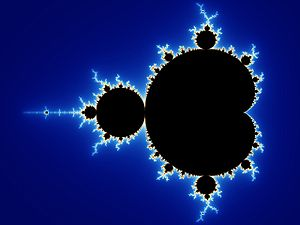
\includegraphics[width=0.8\textwidth]{figures/fractals.jpg}
  \caption{Recursion}
  \label{fig:recursion}
\end{figure}

There is, however, one glaring challenge facing the simulation hypothesis: information capacity and entropy. Simulating even a single strand of human DNA is a daunting computational task, let alone an entire human being. There are over eight billion of us, not to mention countless animals, plants, and microorganisms. Our Milky Way galaxy alone contains hundreds of billions of stars, and astronomers have observed hundreds of billions of galaxies.

Sub-simulations would rapidly run out of memory!

Despite their purely virtual nature, these abstract structures possess fascinating properties.
Subjective pain and joy are profoundly real experiences for conscious beings.
Could there be fundamental modes of feeling that biological evolution has simply not implemented in us yet?
Might we experience them if we ultimately end up in a realm like heaven?

(According to my wife, such undiscovered human experiences could certainly explain my typical behavior--I'm obviously running all of
those procedures simultaneously)

In Arnold Schwarzenegger's film \textit{Last Action Hero}, characters cross back and forth between the real world and a fictional film universe.
I never liked the movie because the premise felt far too absurd to me. Silly me.




\backmatter

\end{document}
